\chapter{CoreASIM Implementation of the INTERLACE Business Logic}
\label{ch:CoreAsimImplementation}

\vspace{-1cm}
\begin{center}
Eduard Hirsch
\end{center}

This chapter is taking a look at the ASIM implementation of the Interlace Project which have been done according to the specifications of D2.1 as well as the refinement specifications of the requirements.

In the previous chapter \ref{ch:CoreAsimIntro} the basis for an environment and code execution has been discussed. Further it will be described here how that environment has been utilized. The following detailed implementation design will show what issues and difficulties had to been taken into account.


\section{Introduction}
\label{sec:impl_intro}

The requirements specifications are the basis for the implementation of an executable ASIM model. That model can be found on GitHub \footnote{https://github.com/InterlaceProject/ASIMSpec} will act as a foundation and test/verification template for further business implementations.

This main part of that document is now focusing on the way the ASIM model actually was implemented and how the missing functional parts of the back-end are realized which is mainly about simulating a simple ledger.

\section{Agents}
\label{sec:impl-agents}

The implementation base is founded on several ASIM-agents which are programmed to act independent and communicate with each other by the base messaging system provided by the ICEF infrastructure.

There are small differences between the available ASIM-agents and they can be, base on their purpose, categorized into the following three groups:

\begin{itemize}
	\item full agents
	\item dynamic agents
	\item non-functional agents
\end{itemize}

\textit{Full agents} are started right away from the beginning. They are processing request or are handling other duties over the environment lifetime. \textit{Dynamic agents} are created during a specific phase of a test and destroyed after that test has been completed. \textit{Non-functional agents} are never started directly and are facilitated for integration into another agent. They are hosting initialization code or helper functions in order to compensate for the missing modularization feature of the ASIM-BSL language.

To get more familiar with the actual ASIM realization an extract of available agents is listed in table \ref{tab:model-agents}. Those may act as a template for extending the scenario applying additional use cases or tests. They are covering the core payment functionality, thus credit as well as debit operations.

\begin{table}[H]
\begin{centering}
\small
{
\begin{tabular}{ r | p{9cm} | l }
\hline
\textbf{Agent}	& Function & Type \\
\Xhline{1.5pt}
$scheduler$				& Scheduling, creating and destroying dynamic agents & full\\[3pt]
\hline
$server$				& Server which talks to the dynamic clients in order to handle payment and ledger specific requests & full\\[3pt]
\hline
$CreditRequestClient$	& Handles a test credit request & dynamic\\[3pt]
\hline
$DebitRequestClient$	& Initiating a test debit request & dynamic\\[3pt]
\hline
$DebitAcknoledgeClient$	& Confirming a test debit request & dynamic\\[3pt]
\hline
$initdata$				& Fake database and back-end initalization code to be included into the \textit{server} agent & non-functional\\[3pt]
\Xhline{1.5pt}
\end{tabular}
}
\caption{\small\textbf{Agent list and their respective functionality}}
\label{tab:model-agents}
\end{centering}
\vspace{-0.5cm}
\end{table}

\section{Execution}

As mentioned in chapter \ref{ch:CoreAsimIntro} the specifications are executed using the ICEF framework. There is has been covered how a JSON ICEF file can be loaded and started. Now details are given how that process is working in depth particular for Interlace specification.

The whole process starts with the main ICEF definition file in the ASIMSpec directory called run.icef by definition and is shown in Listing \ref{lst:interlace-json-spec}. It is illustrating how the different types of agents are included into the simulation. To explain further all agents are located in the directories \textit{casim} together with \textit{casim/clients}. Agent file names are the same as described in table \ref{tab:model-agents} including the suffix ".casim". \textit{casim} contains all full plus their non-functional agents which are joined later on. \textit{casim/clients} hosts all the relevant clients talking to a server. Currently there is one client for a credit request and two clients for a debit request.

\begin{center}
\begin{minipage}{0.8\textwidth}
\small
\begin{lstlisting}[language=json,firstnumber=1,caption={\bf\small ICEF JSON Specification for INTERLACE},captionpos=b,label=lst:interlace-json-spec]
{
    "id": "interlace", 
    "schedulers": [{
        "file": "casim/scheduler.casim",
        "include": [
            "casim/clients/CreditRequestClient.casim",
            "casim/clients/DebitRequestClient.casim",
            "casim/clients/DebitAcknowledgeClient.casim"
        ],
        "start": "true"
    }],
    "asims": [{
        "file": "casim/server.casim",
        "include": [
            "casim/initdata.casim"
        ],
        "start": "true"
    }]
}
\end{lstlisting}
\end{minipage}
\end{center}

When looking closer at the icef definition one can see that there are couple of agents defined inside of a json-array with an attribute called \textit{include}. All agents in that array will be added to the main file. That means that CreditRequestClient, DebitRequestClient and DebitAcknowledgeClient are added to the scheduler and initdata is added to server agent.

\textbf{Important note:} The include syntax is used to append code from a different file to an agent but comes with strings attached. See \ref{sec:impl-include} for further details.

Consequently the loading module will assemble no more than two ASIMs - a scheduler and a server. That assembled JSON String is sent to the manger which is initializing the simulation environment and distributing the clients over the available brappers.

\subsection{Main Agents Tasks}
\label{subsec:impl-agent-tasks}

As mentioned in the beginning of that section two main agents, scheduler and server, are the core of the running environment. Once started both instantly start working. The server listens for messages on the communication channel in order to process potential request and the scheduler is initializing the first test and starting clients which should be active during that particular test. When a client has been initialized it will carry out its assigned duties which will be to assemble a request to the server and handle the resulting query-response traffic. Of course the request types are of different types depending on the current test and the type of the client. When the client is done it is sending a message to the scheduler which will terminate the client.

\subsubsection{The scheduler}\ as quickly introduced before is responsible for spawning new clients which are taking over different tasks. To do so the scheduler is defining various things in advance. First the current tests need to be identified which has been done by creating a universe as well as two location:

\begin{lstlisting}[language=bsl]
	universe TEST_STATE = { START, TEST_CREDIT, TEST_DEBIT }
	controlled currentTest: TEST_STATE
	controlled nextTest: TEST_STATE -> TEST_STATE
\end{lstlisting}

The universe \textit{TEST\_STATE} defines the available test list. \textit{currentTest} is set from the the universe \textit{TEST\_STATE} and is defining the currently executed test. Finally \textit{nextTest} is a function which takes as parameter the current test as type \textit{TEST\_STATE} and gives you as result the next test of the queue which is of the same type. To initialized the predefined locations the following command are executed:

\begin{lstlisting}[language=bsl]
	currentTest := START
	nextTest(START) := TEST_CREDIT
	nextTest(TEST_CREDIT) := TEST_DEBIT
\end{lstlisting}

Now it is possible during the execution of the schedulers main program to transition from one test to the next by

\begin{lstlisting}[language=bsl]
	currentTest := nextTest(currentTest)
\end{lstlisting}

applying the current test to the nextTest function. That can be done as long as the return value of the function is \textit{undef} implying that no other test is left.

For the \textit{current test} a functional location is applied which returns a list of client agent for a given test state which can be defined as follows:

\begin{lstlisting}[language=bsl]
	controlled nextClient: TEST_STATE -> LIST
\end{lstlisting}

That \textit{nextClient} function needs to be setted up during the initialization phase of the agent as well

\begin{lstlisting}[language=bsl]
	nextClient(TEST_CREDIT) := [ CreditRequestClient ]
	nextClient(TEST_DEBIT)  := [ DebitAcknowledgeClient, DebitRequestClient ]
\end{lstlisting}

showing that we have one client for a credit request test and two clients for a debit request. Also important to remember is that rules for a client agent are initially defined in a separate file but as noted already included into the scheduler later by just appending the code. Thus each tested client is absolutely required to have unique names for the \textit{initialization}, the \textit{program} and the \textit{policy} rule \textbf{over all} included files!

Next the missing parts are added up to get the full picture on how the clients are started. In particular in which way the base rules for a dynamic client are defined and how they are finally instantiated and handled during runtime. Listing \ref{lst:impl-sched-core} is illustrating the management of the different clients.

\begin{center}
\begin{minipage}{0.8\textwidth}
\small
\begin{lstlisting}[language=bsl_lst,caption={\bf\small Scheduler core functionality},label={lst:impl-sched-core} ]
	//definition of functional location for getting
	//a function reference for a client name
	controlled initBy: CLIENT -> FUNCTION
	controlled withProg: CLIENT -> FUNCTION
	controlled andPol: CLIENT -> FUNCTION
	
	rule Start = {
		...
		//Setup CreditRequestClient rules
		initBy(CreditRequestClient) := InitCreditRequestClient
		withProg(CreditRequestClient) := ProgramCreditRequestClient
		andPol(CreditRequestClient) := SkipCreditRequestClient
		...
	}
	
	rule Program = {
		...
		//Client rules are defined in clientTemplate script
		if currentTest != undef then seq			
			forall createClient in nextClient(currentTest) do
				createASIM createClient
					initializedBy initBy(createClient)
					withProgram withProg(createClient)
					andPolicy andPol(createClient)
					in activeList(createClient)
					
			activeClients := | nextClient(currentTest) |
		endseq
		...
	}
\end{lstlisting}
\end{minipage}
\end{center}

In that listing we can identify three parts. \textbf{First} the definition of three functions which are taking a $CLIENT$ as parameter and returning a $FUNCTION$ can be observed, namely $initBy$, $withProg$ and $andPol$. That $FUNCTION$ return type can be any rule we have defined inside of the scheduler or inside of the dynamic clients which are included to the scheduler. \textbf{Second} for client $CreditRquestClient$ those three function values are set. So for example it is possible to apply $initBy(CreditRequestClient) := InitCreditRequestClient$ and afterwards to call function $InitCreditRequestClient$ by using  $initBy(CreditRequestClient)()$. \textbf{At last} during the iterative execution of the $Program$ rule the actual starting of the client is process. If a valid test has been selected $nextClient(currentTest)$ provides a list of clients valid during that particular test. The $forall$ loop is walking through that list and using the respective iteration to instantiate the chosen client. This instantiation is done by calling $createASIM$ command and passing the start up rule ($initializedBy$), the main program rule ($withProgram$) and the scheduling policy ($andPolicy$).

In line 27 of listing \ref{lst:impl-sched-core} the count of active clients is stored. That count is reduced by one when a "Done" message has been received by a dynamic client. Also the client is shut down by calling

\begin{lstlisting}[language=bsl]
	destroyASIM clientName
\end{lstlisting}

After the $activeClients$ count has been reduced to $0$ again all clients have terminated and the next test can be covered. To conclude it is possible to say that $activeClients$ count is used as a structure similar to semaphores which is taking care that no new clients are issued as long as it has a value bigger than $0$ and the scheduler is therefore in something similar to a paused state. Certainly, is it not really paused but in a "busy wait loop".

\subsubsection{The server}\ agent is acting as the main component which is implementing most of the specified requirements, which is for the moment credit and debit operations. The server is started right away when CASIMA has received and processed the JSON file for the simulation.

When the init-rule called $Start$ is executed the $Ledger$ and $PendingTransaction$ are initialized as empty maps, an OTP lifetime is set as well as the $Logger$ is setted up. The logger offers several logging levels and details about it can be found in section \ref{sec:impl-log}. Also a rule called $InitData()$ is executed at start-up. It is important to know that the Eclipse Plug-in is showing that this rule is having a Problem/Error because it is not defined in the server.casim file and thus not recognizable for it. Nevertheless, that rule is placed correctly and will work fine, because it is defined in the non-functional agent $initdata$. The content of $initdata$ is, due to the $include$ statement inside of the run.icef, appended to the server.casim before it is sent to the CASIMA manger.

Rule $initData$ in the $initdata$ client is consolidating the rest of the initialization inside. To be more specific the following locations are prepared for later usage when it is called:

\begin{itemize}
	\item $sessionData$ ... simulates session information
	\item $profileTable$ ... contains user profiles
	\item $accountTable$ ... user accounts
	\item $userGroupTable$ ... specifying users group membership
	\item $TT$ ... transfer type translation table
	\item $accountConnectivity$ ... transferability between accounts
\end{itemize}

After the start-up phase has been finished the server is going into listening mode when the main program $DispatchMessages$ is called iteratively. In there all relevant messages received by the server are taken care of. In listing \ref{lst:impl-msg-dispatch} the dispatch process of server can be viewed in detail. All inbox messages of the current engine tick are fetched using the $inboxOf$ in addition to the $forall$ statement. The message reference $m$ as named in the loop is used to retrieve subject, message and sender of the current post box entry $m$.

Messages which are not recognized having an accurate message type are discarded. The message type is defined by the message subject and is compared to one of the predefined entries in the universe definition $MESSAGE\_REQUESTS$. For real world use it is essential to introduce some kind of additional message signing to ensure by whom the message has been sent.

\begin{center}
\begin{minipage}{0.8\textwidth}
\small
\begin{lstlisting}[language=bsl_lst,caption={\bf\small Server message dispatching},label={lst:impl-msg-dispatch} ]
rule DispatchMessages = {
	forall m in inboxOf(self) do seq
		//fetch message information
		msubject := getMessageSubject(m)
		msgIn := getMessageContent(m)
		member := getMessageSender(m)
		
		//dispatch messages
		if msgIn != undef and member != undef then
			case msubject of
				toString(CreditReviewReq): HandleCreditPreviewReq(msgIn, member)
				toString(CreditPerformReq): HandleCreditPerformReq(msgIn, member)
				toString(DebitPreviewReq): HandleDebitPreviewReq(msgIn, member)
				toString(DebitPerformReq): HandleDebitPerformReq(msgIn, member)
				toString(DebitAckCompletion): HandleDebitAckCompletion(msgIn, member)
			endcase
	endseq //end forall
}
\end{lstlisting}
\end{minipage}
\end{center}

\section{Modularization and Include Syntax}
\label{sec:impl-include}

For the Interlace specification the ICEF framework has been extended to support an "include" syntax inside of the ICEF JSON files in order to import sources to an agent. This has been added in order to compensate for the "Modularity" module of ASM which stops working in ASIM because of its distributed nature.

However, it is important to know that the include statement needs to be used with caution, because one need to be aware that it is nothing more but appending the content of the included file to the main agent file. This appending raises the following issues:

\begin{itemize}
	\item Line numbers are different to the original files
	\item For a compilation problem it might be necessary to take a look at all files, main as well as included ones
	\item Naming needs to be consistent throughout all files. E.g. Eclipse will not notify a developer whether a name for a rule, location, ... has been used twice.
\end{itemize}

Nevertheless, it is an approach for handling the code separation in order to avoid a single and extremely long file which would be difficult to maintain and work with.

For being able to use \textbf{Eclipse} and the ASIM eclipse hinting/error detection provided by the plugin another quick fix has been introduced. So if you'd add a dynamic or non-function agent it will be appended at some point to a parent agent. Thus definitions like "CoreASIM asimname" would occur twice inside of that final agent. For the interpreter to work correctly it is consequently necessary to have only one header defining the name of an agent and to remove that header definition inside of the included files. But when you are removing the header definition Eclipse is not able any more to provide correct syntax highlighting, hinting or error detection.

Thus you now have the possibility to mark a section which will be removed during the agent assembling. The beginning of such a section is marked with \textcolor{eclipseComment}{/*includeskip begin*/} and the end with \textcolor{eclipseComment}{/*includeskip end*/}. When using those markers they need to be placed exactly as described - no additional white-spaces (space, tab, return, ...) or different casing. Listing \ref{lst:includeskip} is showing a short example.

Inside of the skipped section there may be many different things placed as shown in the example in order to work seamlessly with the Eclipse hinting. So you could also place names of locations or universes. The reason putting them there is to avoid a warning by the Eclipse plugin that the variable/location has not been defined yet. So in order to check correct spelling and avoid the problems cause by those only getting obvious at interpretation time.

\begin{center}
\begin{minipage}{0.8\textwidth}
%\small
\begin{lstlisting}[language=bsl_lst,caption={\bf\small includeskip usage},label=lst:includeskip]
/*includeskip begin*/
	//this part will be removed
	CoreASIM Company

	use Standard 
	init dummy
	rule dummy = skip
	scheduling NoPolicy
	policy NoPolicy = skip
/*includeskip end*/

//this rule is included to main agent
rule somerule = {
	...
}
\end{lstlisting}
\end{minipage}
\end{center}

\section{Dynamic Clients}
\label{sec:impl-dyn-clients}

This section will elaborate about the dynamic client features and functionalities. It is explained how they are used as well as how they process the information and create the various request. Further, details about the message types is given in detail.

\subsection{Communication and Message passing}
\label{sec:impl-com-msg}

As mentioned in chapter \ref{ch:CoreAsimIntro} section \ref{sec:coreasim-details} communication in the ICEF framework is based on message passing. Thus each agent has the possibility to send messages to a named agent as well as receive message from any other. Those can be picked up at the agent specific mailbox using the designated functions provided by the communication Plug-in.

All agents work independent, do not share state between each other and only are aware of their own status. Consequently, they have to rely on that mailing system to share information. This is an important fact because in a real-world scenario clients are also working independent from each other. In order to support that independence ASIM agents are applying that distributed design pattern.

Messages from one client to another are not encrypted. Thus it is important to realized that security needs to be taken into account separately and is currently not part of the implemented model but very important when planning a business-ready product.

\subsection{Message Types}
\label{subsec:impl-msg-types}

At the moment there are several message types part of debit and credit requests. Table \ref{tab:impl-transfer-types} is giving an overview which messages are in use for handling transfer operations. The messages are listed in the order of occurrence, however, the precise overall communication sequence is shown in figure \ref{fig:impl-msg-crc} and figure \ref{fig:impl-msg-drc}. Finally, the listed message types in table \ref{tab:impl-msg-generic-types} are operation (debit, credit) agnostic but vary based on their transfer parameters.

\begin{table}[H]
\begin{centering}
\small
{
\begin{tabular}{ r | p{7cm} | p{4cm} }
\hline
\textbf{Message Name} & Used For & Attached Parameters \\
\Xhline{1.5pt}

CreditPreviewReq & first check of \textbf{credit} request & CRP$^{*}$ \\[3pt]
\hline
CreditPerformReq & request to actually perform a \textbf{credit} request & CRP$^{*}$ \\[3pt]
\Xhline{1.5pt}
DebitPreviewReq & first check of \textbf{debit} request & DRP$^{**}$ \\[3pt]
\hline
DebitPerformReq & request to actually perform a \textbf{debit} request & DRP$^{**}$ \\[3pt]
\hline
ConfirmationReq & asking debitor for permission to perform that \textbf{debit}-transfer & DRP$^{**}$, OTP$^{***}$ \\[3pt]
\hline
DebitAckMsg & debitor gives permission to perform that \textbf{debit}-transfer & DRP$^{**, 1}$, OTP$^{***}$ \\[3pt]

\Xhline{1.5pt}
\end{tabular}
}
\caption{\small\textbf{Credit/Debit message types overview}\\
($^{*}$Credit Request Parameters: from-account, to-account, amount, meta-data, channel, member)\\
($^{**}$Debit Request Parameters:  creditor, debtor, amount, meta-data, channel)\\
($^{***}$One Time Pad, $^1$optional)}
\label{tab:impl-transfer-types}
\end{centering}
\vspace{-0.5cm}
\end{table}


\begin{table}[H]
\begin{centering}
\small
{
\begin{tabular}{ r | p{7cm} | p{3.1cm} }
\hline
\textbf{Message Name} & Used For & Attached Parameters \\
\Xhline{1.5pt}

ProceedMessage & answer from server that the CreditPreviewReq has been successful & CRP$^{*}$/DRP$^{**}$\\[3pt]
\hline
DoNotProceedMessage & answer from server that the CreditPreviewReq has NOT  been successful & error-text, CRP$^{*}$/DRP$^{**}$\\[3pt]
\hline
NoPermitted & answer from server that the CreditPerformReq has NOT  been successful & error-text, CRP$^{*}$/DRP$^{**}$ \\[3pt]
\hline
TransferPerformedSuccessful\ & answer from server that the CreditPerformReq has been successful and the transfer has been recorded and confirmed & success-message, CRP$^{*}$/DRP$^{**}$ \\[3pt]
\hline
Done & Message to Scheduler the client simulation is done and can be terminated & none \\[3pt]

\Xhline{1.5pt}
\end{tabular}
}
\caption{\small\textbf{Operation agnostic message types overview}\\
($^{*}$Credit Request Parameters: from-account, to-account, amount, meta-data, channel, member)\\
($^{**}$Debit Request Parameters:  creditor, debtor, amount, meta-data, channel)}
\label{tab:impl-msg-generic-types}
\end{centering}
\vspace{-0.5cm}
\end{table}

Lets review the implementation of a credit review request to a running agent called "server" in listing \ref{lst:impl-msg-send}. When taking a closer look at line 9 it can be observed that the $send$ command is setting a location named $CREDITREQUEST$ for the message content and one called $CreditReviewReq$ is used for defining the message subject.

$CREDITREQUEST$ is of type map, which is used in BSL/ASM language as a set of key/value-pairs. That map carries the information required for that message type, implying that for the credit transfer example in listing \ref{lst:impl-msg-send} the parameters are chosen accordingly (see CRP in table \ref{tab:impl-transfer-types}).

The actual message type is determined by the subject. As mentioned $CreditReviewReq$ content is used for defining the subject. At client level, unfortunately, it is not possible to predefine a universe containing the $CreditReviewReq$ like done in the head section of the server. The reason is that the $createASIM$ command used in the scheduler for spawning dynamic clients does not allow to include a header section, just an init rule, the main program and finally the scheduling policy. The consequence is that the used message types for clients are locations of type $STRING$ which are created in the init rule and setted up as locations having same name like their values. See line 1 in listing \ref{lst:impl-msg-send}.

\begin{center}
\begin{minipage}{0.8\textwidth}
\small
\begin{lstlisting}[language=bsl_lst,caption={\bf\small send message},label={lst:impl-msg-send} ]
	CreditReviewReq := "CreditReviewReq"
	CREDITREQUEST := {
					"from" -> "accId1",
					"to" -> "accId2",
					"channel" -> "Service",
					"amount"  -> 2000,
					"metadata" -> {"message", "some transfer"}
				}
	send CREDITREQUEST  to "server" with subject CreditReviewReq
\end{lstlisting}
\end{minipage}
\end{center}

Concluding further the subject containing the message type is always converted to $STRING$ type in order to stay consistent. Also server agent, which is using a universe definition, is converting its enumerative representation of message types to $STRING$ by calling $toString(CreditReviewReq)$ when sticking to the example of credit review request.

The reason for naming locations exactly after their content is based on a programmers principle which says that strings which are static and never change should be represented by a fix variable term or in ASM/BSL language terms as a predefined location. That best-practices principle has the following benefits:

\begin{itemize}
	\item Typing errors can be immediately found because an IDE\footnote{Integrated development environment} usually shows them as unknown or undefined. Whereas a misspelled text might be only found during runtime.
	\item Known variables/locations can be facilitated during syntax completion and therefore simplify and speed up the implementation process.
	\item It is easyer to find states which still need to be taken care of on other places.
	\item Usage of specific types might be restricted under certain conditions.
\end{itemize}

\subsection{Client Features and Functionalities}
\label{subsec:impl-client-features}

For Interlace, and of course for any other software project, it is important to test its correctness. This document will not talk about those tests but covers details on how clients are prepared to support a testing environment. These clients will be later facilitated to act like user devices performing a specific action or transfer.

That clients are called "dynamic" due to their limited lifespan and are as of section \ref{sec:impl-agents} not intended to be started right with the begin of the Interlace simulation but rather in terms of an on-demand need. Thus, their lifespan is meant to be restricted to the duration of their specific task.

To perform those tasks similar to a user-device-action an additional layer has been introduced which was not part of the requirements definitions. That layer explained in detail in section \ref{sec:impl-login-layer} adds a pseudo-login possibility and holds session-similar information for each created client by the scheduler. Thus in terms of network-topology the name of an ASIM is defined as the address of a device and the (member-)name of a user can be looked up inside a session table.

\begin{figure}[htbp]
  \centering
  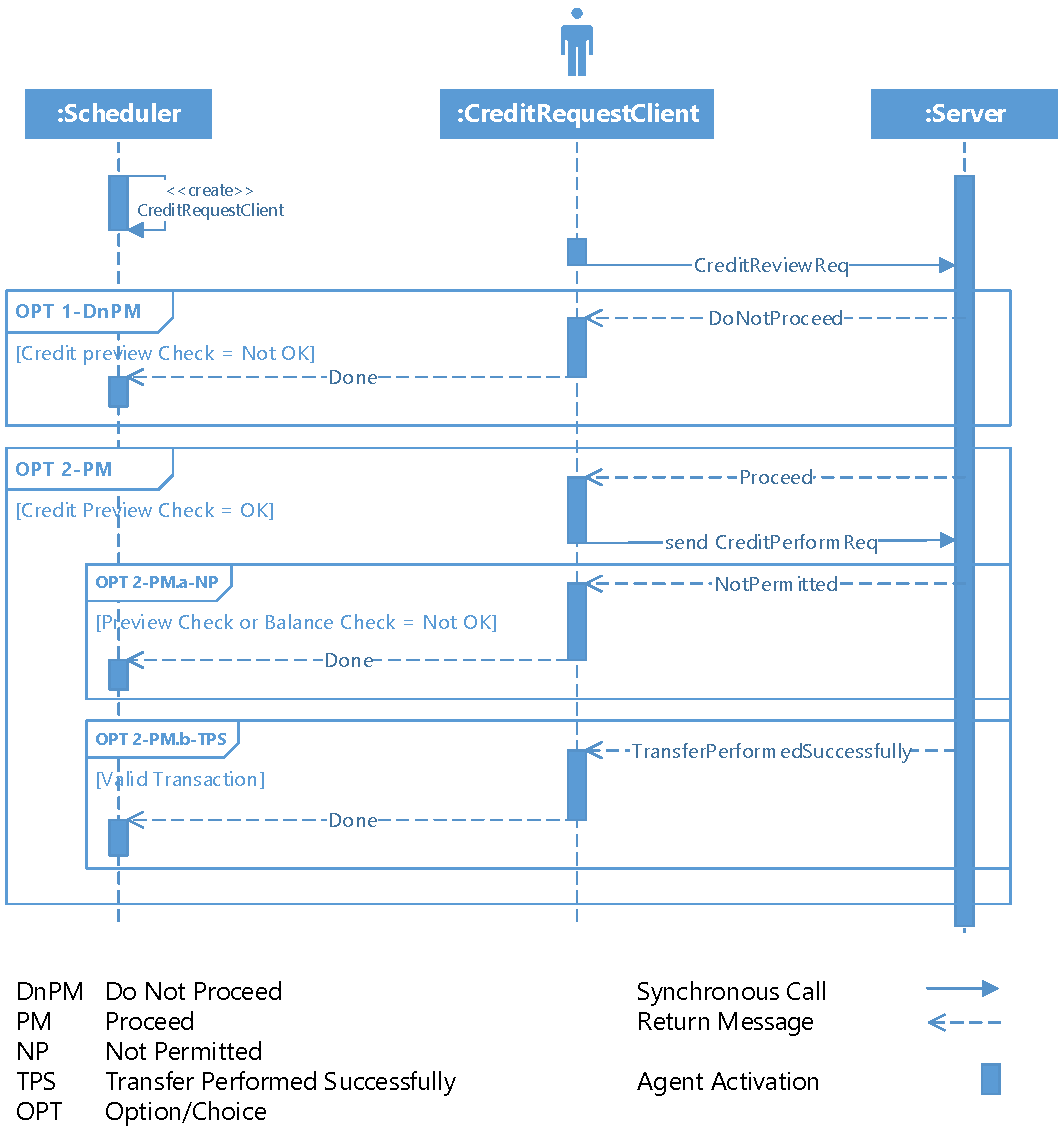
\includegraphics[width=1.0\textwidth]{Figures/creditrequest}
  \caption{\bf\small Credit request message protocol}
  \label{fig:impl-msg-crc}
\end{figure}

When following the sequence diagram in \ref{fig:impl-msg-crc} it is necessary to keep in mind that these messages are send from a $CreditRequestClient$ but initiated and owned by a member which is logged in and registered in the session data lookup table. For the server agent process it is important know which member is currently sending that transfer in order to perform various checks and store valid transfers. Certainly, same applies for the $DebitRequestClient$ and the $DebitAcknowledgeClient$ of figure \ref{fig:impl-msg-drc}.

\textbf{Dynamic Request Clients} start off when being created by the $scheduler$ agent and don't send or receive any request beforehand. According to a typical state machine the clients manage their own states and acting along them. CRC\footnote{Credit Request Client} and DRC \footnote{Debit Request Client} are using four main states which are explained in detail in \ref{subsec:impl-states}.

The message sequence from client to server is specified in \ref{fig:impl-msg-crc} for the CRC-client and in \ref{fig:impl-msg-drc} for the DRC-client. When investigating those two figures it is standing out that the message sequence looks very similar, only the names vary by their prefix (debit versus credit). However, what might not be obvious here is that the request parameters are quite different.

Another main difference between credit and debit message sequence is though, that a debit request needs $ConfirmationReq$ as well as $DebitAckMsg$. This is necessary because a initiating creditor (seller) needs to have the transaction confirmed by the debtor (buyer) to be sure having a valid transaction which is crediting the payment to the sellers own account.

\begin{figure}[htbp]
  \centering
  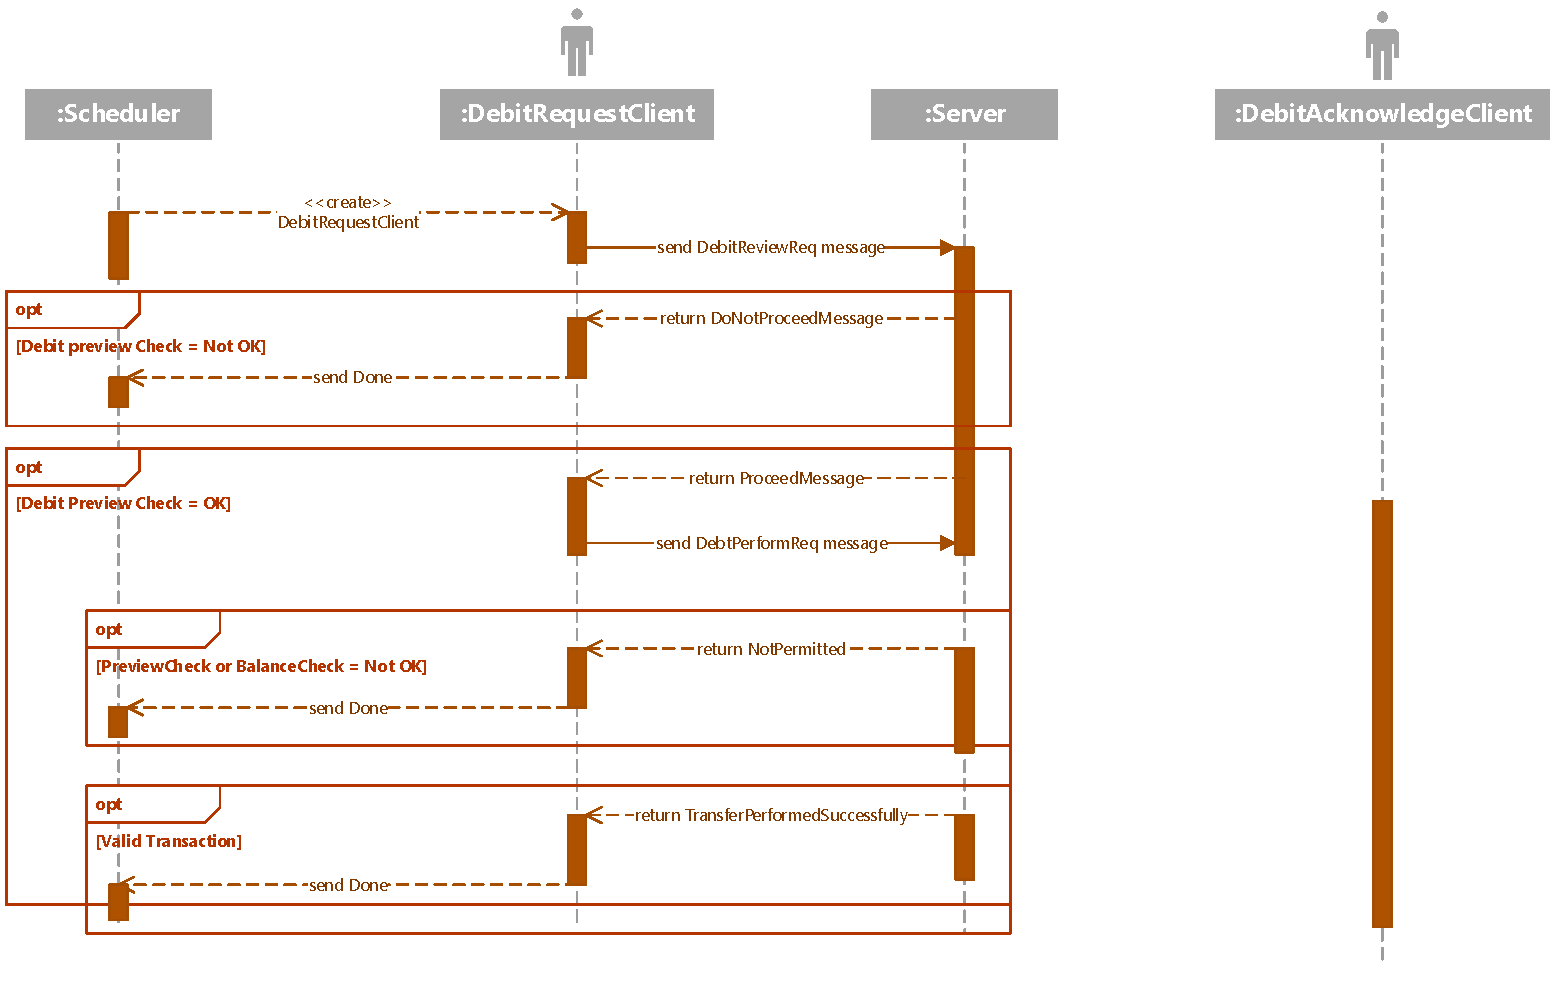
\includegraphics[width=1.0\textwidth]{Figures/debitrequest}
  \caption{\bf\small Debit request message protocol}
  \label{fig:impl-msg-drc}
\end{figure}

The sequence diagrams denote optional flows using option boxes. These boxes are having a unique numbered name. An option $OPT$ at the first level has a number (choice $1$ or $2$) as well as an abbreviated name ($DnPM$, $PM$). Sub-options in the second level are alphabetically numbered and also followed by an abbreviated name. Squared brackets underneath the option name indicate the current option choice.

ASIMs currently do not have the possibility to sleep for some time or until an event has occurred. Nevertheless, agents are able to reduce the executed command in the current tick to a minimum achieving a similar result. Inside of the sequence diagrams activated clients are shown by the vertical fully colored bars. Non-active phases are indicated by the vertical dashed lines.

The emulated users in the figures are pictured on top of the clients to show that request are send by particular member.

Scheduler and server are agents which can be seen as autonomous processes in the simulation. The scheduler mainly acts as an orchestration tool for testing purposes and will be removed for actually deployed applications whereas the server agent needs to exist in a real-world scenario. Maybe not as a process running on a centralized server structure but when taking a real distributed scenario into account it'll be implemented using some kind of smart contract running inside of a virtual machine in a blockchain-environment.

\subsection{State Management}
\label{subsec:impl-states}

\subsubsection{Client States}\ are managed over four predefined pseudo-static locations which are as following

\begin{itemize}
	\item SEND: only sending message
	\item RECEIVE: receive and directly respond to messages
	\item TERMINATE: end execution; send "Done" message
	\item DONE: everything is done; ready to be terminated
\end{itemize}

$SEND$ might be used if a sequence of messages will be sent were no replay message is needed or just to submit an initial message at start-up before going right into the $RECEIVE$-mode.

$RECEIVE$ waits for the messages and act accordingly. When a message has been received and it is necessary to send a response it is done right in $RECEIVE$-mode without changing to $SEND$-mode.

$SEND$ and $RECEIVE$ state could be set alternately but when state $TERMINATE$ is applied the process of shutting down the agent has been started. Once $DONE$-state is reached, even if not stopped yet by the scheduler, the client won't do anything useful any more.

The DAC\footnote{Debit Acknowledge Client} uses the same states except for the $SEND$-state because it only needs to receive and confirm a transfer by using the given one time pad. The DAC is an example that not all of the states need to covered by a client which might be of interest when creating new clients.

\subsubsection{Server \& Scheduler States}\ are not particular part of that section about the dynamic clients, nevertheless, a brief explanation of their states is given.

\textbf{The server} does not have any particular mode or state management yet. It is just waiting for messages and when receiving one it will be directly processed.

\textbf{The scheduler} mainly has its test states and is transitioning from one test to another till there are no tests left. For each test the scheduler has two stages. First in a starting phase all clients are started and counted. Then the scheduler in its second phase waits for as many $DONE$-messages like clients have been issued. Finally the scheduler goes to the next test and starts that two-phase process again.

%%%%%%%%%%TODO%%%%%%%%%
\section{Logging}
\label{sec:impl-log}

server logger


\section{Simple Test Scenario}
\label{sec:impl-test}

explain test cases and scenarios

\section{Database and Agent Initialization}
\label{sec:impl-db-init}

init data
temp table structure
backend simulation

\section{Additional Login Layer}
\label{sec:impl-login-layer}

active login how handled

\section{Important Rule}
\label{sec:impl-rules}

explain helper rules not defined in requirements nor in other sections

\section{Issues}
\label{sec:impl-issues}

function conversion/translation, bugs?? brief, reference to correction

what is implemented, what is missing, centralized architecture (message passing??)